\section{Comparison of Simulation Results with Data}
  \label{sec:simultons_results}

    In the previous section we built up a theoretical model for the physical
    system, including the significant effects of motion and atomic structure, and
    presented numerical simulations using parameters matching those of the
    experiment described in section \ref{sec:simultons_experiment}. We'll now
    compare the results of those simulations with the experimental data.

    \begin{figure}[h]
      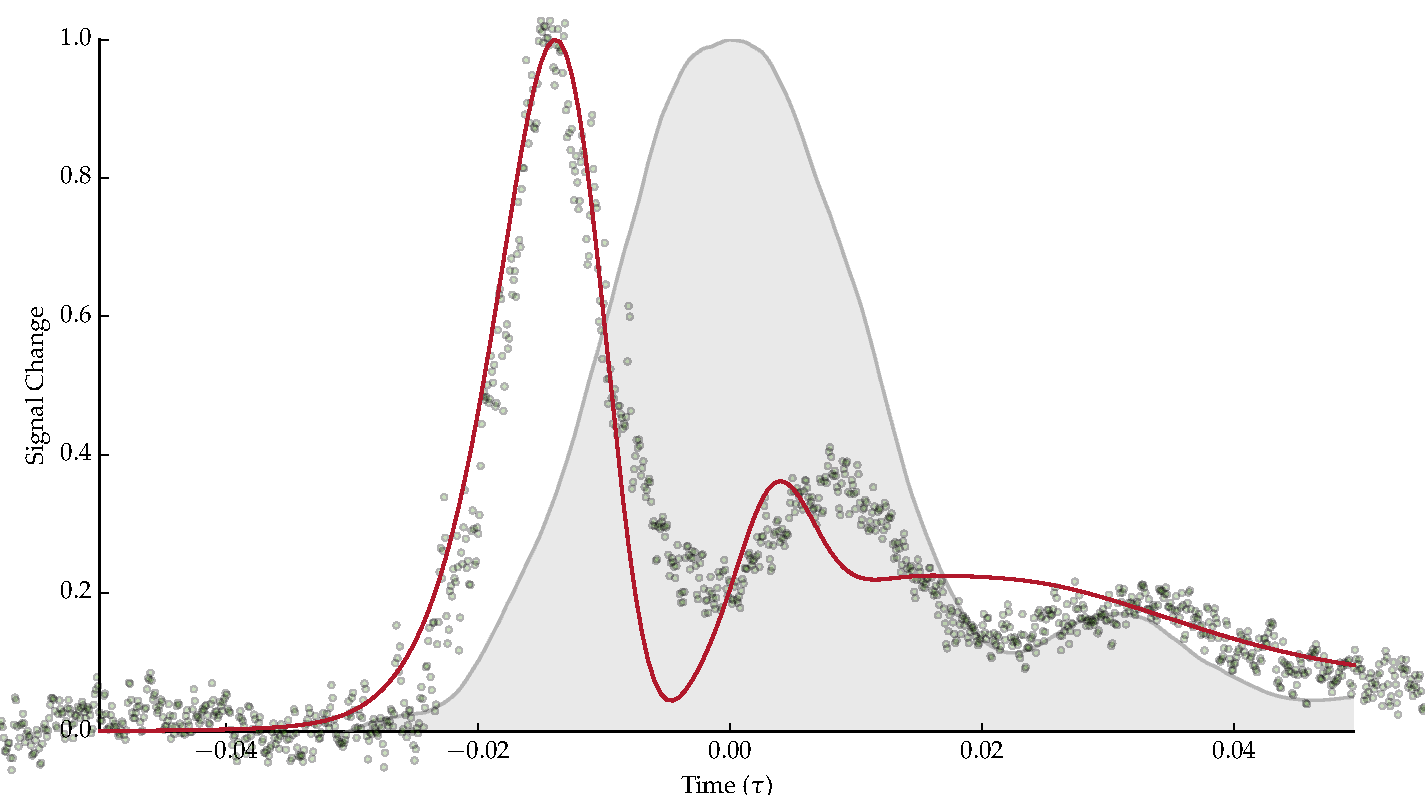
\includegraphics[width=\linewidth]{figs/06_simultons/mb_vee2g_15c_130p_0330t_230C_sb50_120vel010_10_002um_fig1.pdf}
      \caption{
      Comparison of normalised probe transmission profiles from the  laboratory
      data (green circles) and simulation results (red line) for an  experiment
      in the \textsc{cw}/pulse scheme. The measured input coupling  pulse
      intensity (grey filled area) has a width $t_w = $ \unit[$0.80$]{ns}  $
      \equiv $ \unit[$0.029$]{$\tau$}, a peak power of \unit[$85$]{mW}  and is
      centred at zero. In this example $T = \unit[230]{\textrm{\textdegree C}}$
      and $L = $ \unit[$2$]{$\mu$m}.
      }
      \label{fig:sim_data_0703_temp_210C}
    \end{figure}

    In figure \ref{fig:sim_data_0703_temp_210C} we present again an example of
    the response in the probe signal (green circles) as a result of the medium
    being disturbed by the coupling pulse (grey filled area). In this case the
    temperature $T = \unit[230]{\textrm{\textdegree C}}$, the length of the
    vapour cell $L =$ \unit[$2$]{$\mu$m} and the peak pulse power is
    \unit[$85$]{mW}. In contrast to figure \ref{fig:data_1704_temp_201C}, the
    probe signal is normalised to unity. Overlaid on the data for comparison
    this time is the simulation result (red line). The simulated coupling pulse
    matches the experimental width of $t~=$~\unit[$0.029$]{$\tau$}.

    The only fitted parameter in the simulation is the peak Rabi frequency of the
    coupling pulse envelope. As we shall see when we look at power dependence, the
    peak Rabi frequency of the coupling pulse determines the arrival time of the
    signal response. We here use the arrival time of the experimental signal to fit
    a simulated peak Rabi frequency $\Omega_c = \unit[2\pi~130]{\Gamma}$.

    A low-pass filter is applied to the simulation result to account for a limit
    in resolution of the photon detector of \unit[$2\pi \cdot 8$]{GHz}. This is effected by a Fourier transform of the intensity profile in the time
    domain to the frequency domain and removal of frequencies $\lvert \omega
    \rvert > \omega_c$ before an inverse transform is made back to the time
    domain. A sharp cutoff would introduce discontinuities, so instead we apply a
    convolution with a roll-off frequency curve
    \begin{equation}
        f(\omega) = \frac{1}{\sqrt{1 + 
                      \left( \frac{\omega}{\omega_c} \right)^2}}.
    \end{equation}

    We see good qualitative agreement with the data. The simple three-level model
    result shows the distinctive steep rise in the probe transmission, the early
    peak around $t = $ \unit[$-0.015$]{$\tau$} followed by a subsequent, smaller
    oscillation. The smaller peak arrives early in the simulation, and is narrower
    than in the data. Both experiment and simulation show the signal returning to
    its original level beyond $t = $ \unit[$0.04$]{$\tau$}.

    The additional `bump' in the pulse profile is the likely cause of a
    following oscillation in the probe signal. This artefact is not included in
    the simulation is not observed in the probe signal tail.

  \subsection{Power Dependence}

    \begin{figure}[p]
    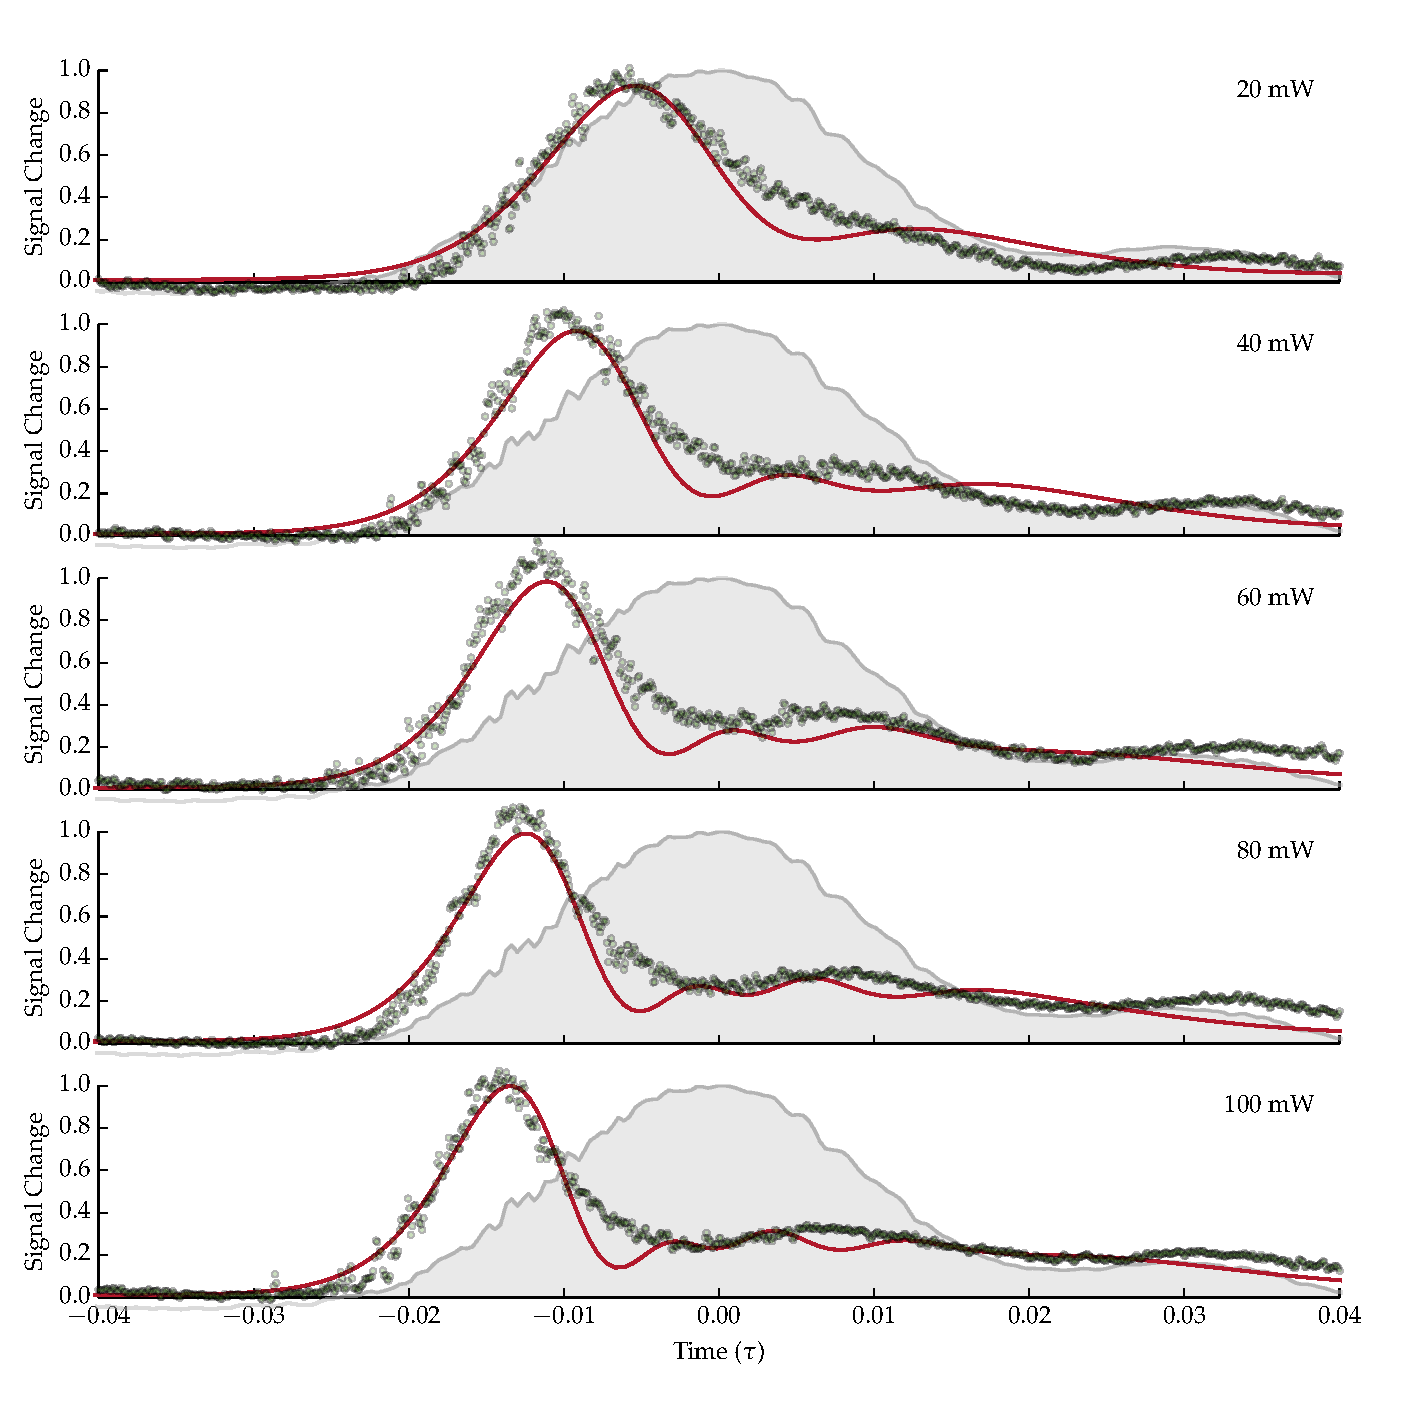
\includegraphics[width=\linewidth]
      {figs/06_simultons/solve_b_multi_01_fig1.pdf}
    \caption{
    Comparison of numerical results (red) with experimental data (green circles)
    for the normalised transmitted probe signal at $L~=$~\unit[$2$]{$\mu$m} over
    a range of peak coupling pulse powers. The measured coupling pulse signal
    (grey filled area) has a width $\tau_w = $ \unit[$0.80$]{ns} $ \equiv $
    \unit[$0.029$]{$\tau$} in each case, and the \unit[100]{mW} pulse envelope
    is shown in each subfigure. The temperature is fixed at
    \unit[$200$]{\textdegree C}.
    } 
    \label{fig:exp_result_power_dep} 
    \end{figure}
    In figure \ref{fig:exp_result_power_dep} we present results for the probe
    transmission signal over a range of experimental coupling pulse powers from
    \unit[20]{mW} to \unit[100]{mW}. The input pulse in each case has a
    \textsc{fwhm} of \unit[$0.80$]{ns}, equivalent to $\tau_w = $
    \unit[$0.029$]{$\tau$} in the natural unit system.

    As discussed in section \ref{sec:simultons_experiment}, the effective probe
    and coupling Rabi frequencies for the atom-light interaction in the cell is
    difficult to determine due to the focussing effect of the cell windows. The
    peak Rabi frequency in the simulation is therefore fitted for that of the
    \unit[100]{mW} data, at $\Omega_c = \unit[2\pi~140]{\Gamma}$.  This value is
    approximately half of that which we calculate directly from the laser power,
    beam waist and transition dipole matrix element for $^{85}$Rb. The
    difference is reasonable if we take into account our uncertainty in the
    field amplitude at the site of the atoms due to beam focussing as well as
    the effective \textsc{tdme} due to hyperfine degeneracy (we will discuss
    this in section \ref{sec:simultons_long}). The Rabi frequencies for other
    input intensities are derived from the \unit[100]{mW} value, following the relationship $\Omega \propto \sqrt{I}$.

    The simulation and experimental data are normalised to the peak intensity in
    response to the \unit[100]{mW} run. The response peaks at lower powers are
    reduced in the data, to $0.93$ in the \unit[20]{mW} run. This is matched in
    the simulation. The key feature of increasing power is to \textit{push the
    response peak earlier} relative to the coupling pulse, from around
    \unit[$-0.08$]{$\tau$} for the \unit[20]{mW} run to \unit[$-0.15$]{$\tau$}
    for the \unit[100]{mW} run, and to \textit{steepen} the peaks. The
    simulation results also match this behaviour over the power range
    investigated.

  \subsection{Temperature Dependence}

    \begin{figure}[p]
    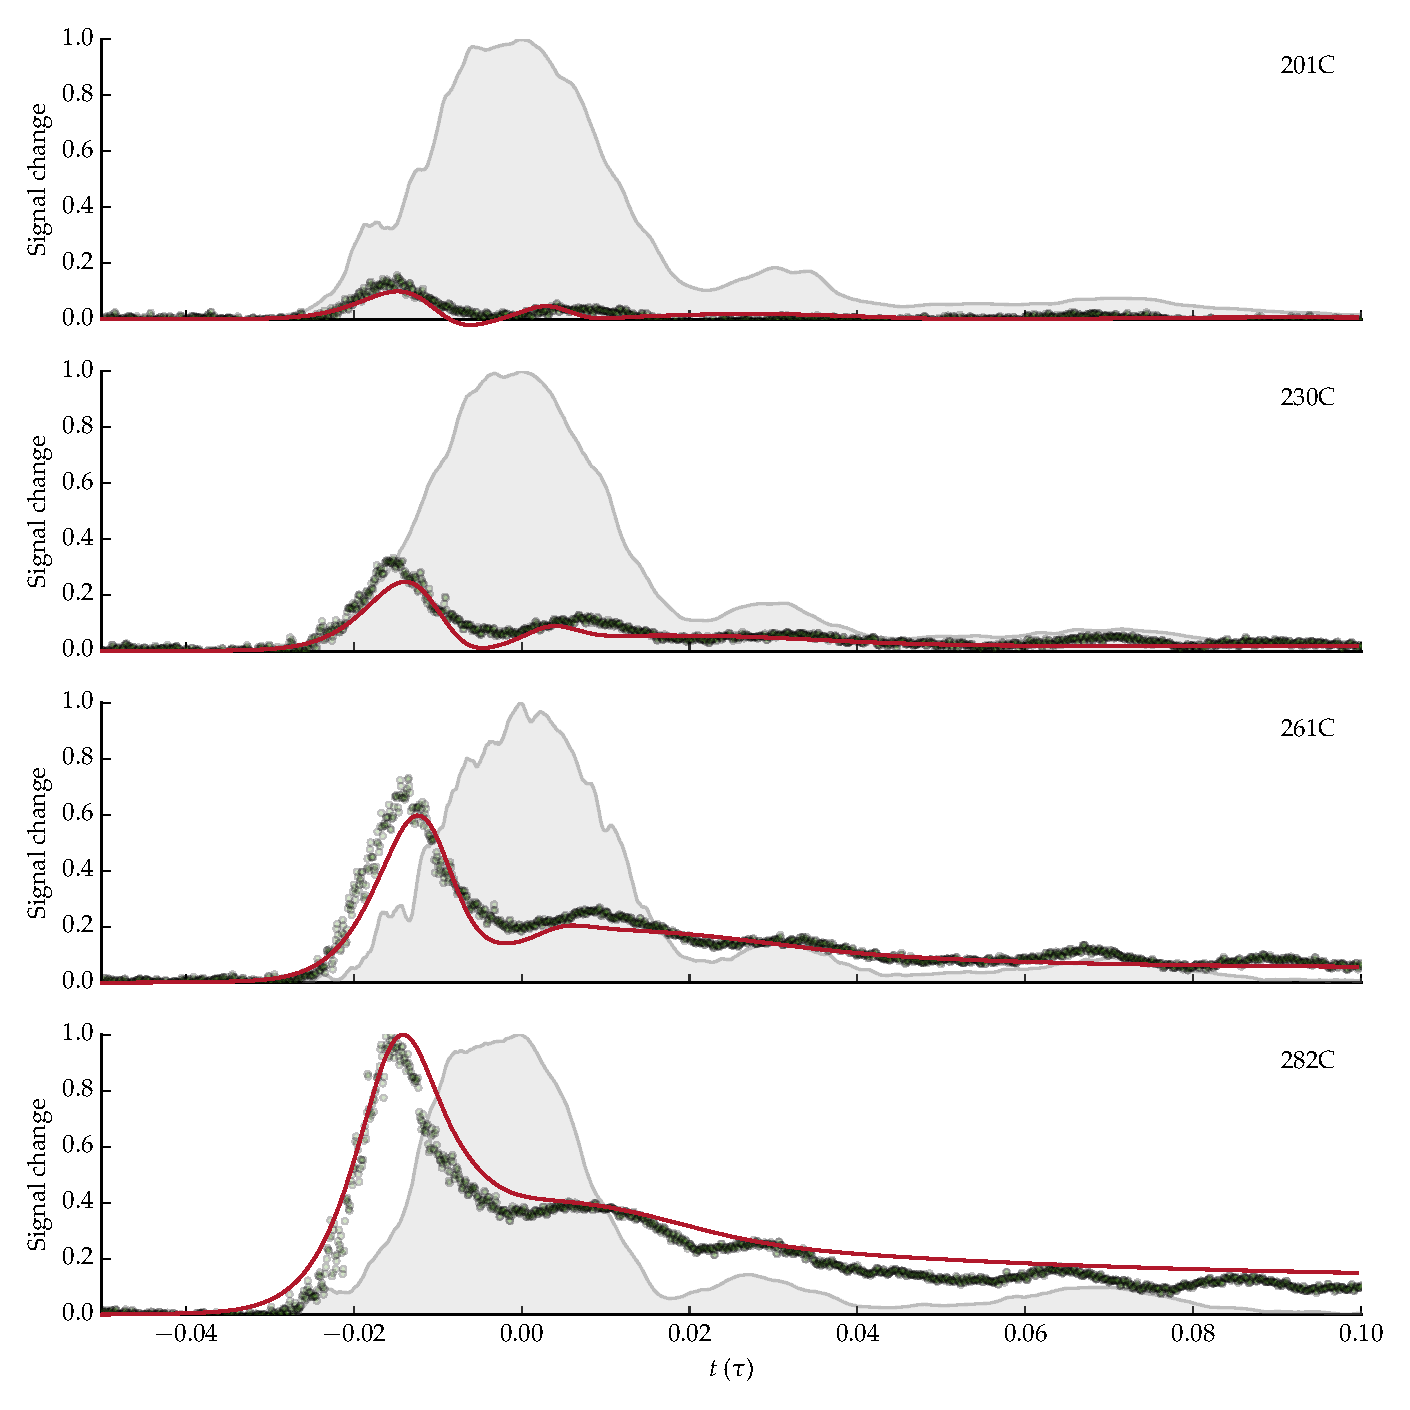
\includegraphics[width=\linewidth]{figs/06_simultons/mb_vee2g_exp_plot_temp_282_fig1.pdf}
    \caption{
    Comparison of numerical results (red) with experimental data (green circles)
    for the transmitted probe signal at $L~=$~\unit[$2$]{$\mu$m} over a range of
    temperatures from \unit[$200$]{\textdegree C} to \unit[$282$]{\textdegree
    C}. The signals are normalised to the peak of the \unit[$282$]{\textdegree
    C} data. The normalised measured coupling pulse signal (grey filled area),
    shown for comparison, has a width $\tau_w = $ \unit[$0.80$]{ns} $ \equiv $
    \unit[$0.029$]{$\Gamma$} in each case. The coupling pulse power is
    \unit[$85$]{mW}.
    } 
    \label{fig:exp_result_temp_dep} 
    \end{figure}

    In figure \ref{fig:exp_result_temp_dep} we present numerical results for the
    probe transmission signal in the time window around the pulse ($t\!=\!0$)
    over a range of temperatures from \unit[$200$]{\textdegree C} to
    \unit[$282$]{\textdegree C}. These simulated results are shown on top of the
    experimental data for comparison, and the measured coupling pulse for each
    run is shown (normalised) for reference on the time axis.

    We see that there is good qualitative agreement between the simulated result
    and experimental data across the temperature range. The increase in
    temperature does not significantly affect the peak time of the response
    signal, but does linearly increase the peak intensity, and this is matched
    in the simulation. The behaviour of the probe after the pulse has passed is
    also in reasonable agreement, though there are clear oscillations in the
    data which are not matched in the simulation.

  \subsection{A Recap}

    At this point we have built up a theoretical model based on propagation of
    the fields through a V-type three-level medium, considering important
    physical effects of inhomogeneous broadening, binary collisions and
    hyperfine pumping. We've chosen appropriate parameters to compare simulation
    results with the experimental data and observe a good qualitative fit across the power and temperature parameter space covered in the laboratory study.

    Having some trust that our model is useful in matching the experiment, we'd like to gain physical insight into the underlying mechanisms responsible
    for the observed data. We begin by looking more closely into the response of an individual atom to the applied fields.
